\usetikzlibrary{automata, positioning, arrows}
\tikzset{
    ->, % makes the edges directed
    >=stealth, % makes the arrow heads bold
    node distance=3cm, % specifies the minimum distance between two nodes. Change if necessary.
    every state/.style={thick}, % sets the properties for each ’state’ node
    initial text=$ $, % sets the text that appears on the start arrow
}

\chapter{Context Free Grammars}

We saw that Turing Machines are able to compute any computable function. However, they have a significant limiitation in that they cannot reason about themselves in meaningful ways. Even further, it can sometimes be considered a bug to be Turing Complete, as seen in the case of the Ethereum Contract language Solidity. Hackers can take advantage of Turing Completeness! For these reasons, sometimes a more limited model of computation is desirable. Context Free Grammars are one such model. Compared to DFA's and TM's, CFG compututational power ranks as follows:

\[
    \text{DFA}  < \text{CFG} < \text{TM}
\]

\begin{definition}
    
    We define a grammar $G$, with variables $V$, terminal symbols $\Sigma$, rules $R$, and start variables $S$. $V$ is disjoint from $\Sigma$.

    \[
        G = (V, \Sigma, R, S) 
    \]

    Rules are defined as follows. They go from variables to terminal symbols and other variables.
    \[
        R: V \rightarrow \Sigma \cup V
    \] 
\end{definition}

Consider a grammar, $G_1: (\{A\}, \{0, 1\}, R, A)$ with the following rules

\begin{gather*}
    A \rightarrow 0A1 \\
    A \rightarrow \varepsilon \\
\end{gather*}

We can \kw{derive} a string based on our rules. Consider $\alpha \in (\Sigma \cup V)^*, \beta \in (\Sigma \cup V)^*$. We say $\alpha \xRightarrow[G]{} \beta$ if we can get $\beta$ by replacing a variable in $\alpha$ using a rule from R.

The following are valid derivations for $G_1$.
\begin{itemize}
    \item $A \xRightarrow[G_1]{} 0A1$
    \item $0A \xRightarrow[G_1]{} 00A1$
    \item $00A1\xRightarrow[G_1]{} 000A1$
    \item $00A1 \xRightarrow[G_1]{} 001$
    \item $AA0 \xRightarrow[G_1]{} 0A1A0$
    \item $AA0 \xRightarrow[G_1]{} A0A10$
\end{itemize}

We say $\alpha \xRightarrow[G_1]{}^* \beta$ if there exists a \kw{chain of derivations} to get $\beta$ from $\alpha$. In otherwords, there exists some $\alpha_1, \alpha_2, ..., \alpha_{R - 1}$ such that $\alpha \xRightarrow[G]{} \alpha_1 \xRightarrow[G]{} \alpha_2 \xRightarrow[G]{} \alpha_3 \xRightarrow[G]{} ... \xRightarrow[G]{} \alpha_{R-1} \xRightarrow[G]{} \beta$.

\begin{definition}
    
    If $G$ is a grammar, $x \in \Sigma^*$ is matched to $G$ if $S \xRightarrow[G]{}^* x$.
    We say $L_G = \{ x \in \Sigma^*: \text{x matches G}\}$ and $F_G: \Sigma^* \rightarrow \{0, 1\}, F_G(x) = 1$ iff x matches G.

    We say a function $f: \Sigma^* \rightarrow \{0, 1\}^*$ is \kw{context free} if there exists a grammar G such that $f(x) = F_G(x) \forall x$.
\end{definition}

\begin{example}
    
    $G_1: (\{A\}, \{0, 1\}, R, A)$ with the following rules

    \begin{gather*}
        A \rightarrow 0A1 \\
        A \rightarrow \varepsilon \\
    \end{gather*}

    What is the language $L_{G_1}$? Answer: It's $0^n1^n$ for $n \ge 0$. Since the starting variable is $A$, we can only ever add two bits at time (a 0 and a 1). So there must be an equal number of 0's and 1's. 

    Recall, we saw earlier that this is not a regular language. So context free grammars must be more powerful than DFA's. 
\end{example}

\begin{example}
    $G_2: (\{A\}, \{0, 1\}, R, A)$ with the following rules

    \begin{gather*}
        A \rightarrow \text{0A0 | 1A1 | 0 | 1 | }\varepsilon
    \end{gather*}

    $G_2$ generates the language that accepts all palindromes. 
\end{example}

\begin{example}
    $G_3: (\{S\}, \{``(",``)"\}, R, S)$

    \begin{gather*}
        S \rightarrow \text{(S) | SS | } \varepsilon 
    \end{gather*}

    This generates the language with all well matched parenthesis expressions.
\end{example}

\subsection*{Why CFG's?}
All programming languages use CFG's for syntax checking. For every programming language there exists a grammar that generates syntactically valid programs.

We saw before that non regular languages can be context free. However, we can take this a step further and claim that CFG's are \emph{strictly} more powerful than DFA's.

\begin{theorem}
    
    Every regular language is also context free. For every DFA D, there exists a CFG G such that $D(x) = F_G(x) \forall x$.
\end{theorem}

\begin{proof}
    
    We can prove this by construction. The goal is a grammar that emulates the behaviour of the DFA i.e. with the same input, the function output is the same.
    \begin{itemize}
        \item Create a variable for each state
        \item The starting variable is $V_0$, the first state
        \item For each transition $T(i, a) = j$, add a rule $V_i \rightarrow aV_j$
        \item For each accepting state i, add $V_i \rightarrow \varepsilon$
    \end{itemize}
\end{proof}

\begin{example}
    \begin{center}
        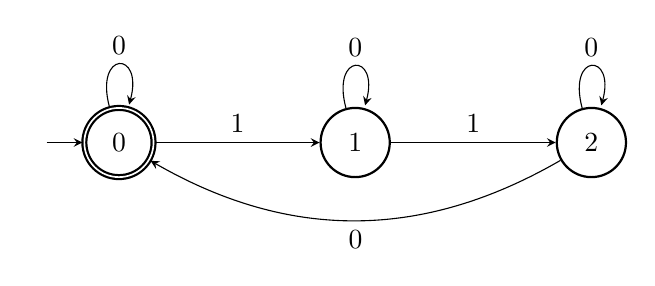
\begin{tikzpicture}
            \node[state, initial, accepting] (q0) {0};
            \node[state, right of=q0] (q1) {1};
            \node[state, right of=q1] (q2) {2};

            \draw (q0) edge[loop above] node{0} (q0)
                  (q0) edge[above] node{1} (q1)
                  (q1) edge[loop above] node{0} (q1)
                  (q2) edge[loop above] node{0} (q2)
                  (q1) edge [above] node{1} (q2)
                  (q2) edge[bend left, below] node{0} (q0);
        \end{tikzpicture}
    \end{center}

    For the equivalent grammar, $\Sigma = \{0, 1\}, V = \{ V_0, V_1, V_2 \}, S = V_0$. 

    Rules$:$
    \begin{gather*}
        V_0 \rightarrow 0 V_0 | 1 V_1 | \varepsilon \\
        V_1 \rightarrow 0 V_1 | 1 V_2 \\
        V_2 \rightarrow 0 V_2 | 1 V_0 \\
    \end{gather*}
\end{example}

To go from NFA's to CFG's we perform a similar construction. Every transition has a rule with the seen bit preceeding the next state (including epsilon transitions, where the seen bit is the empty string).

\section{Designing CFG's}
When thinking about how to design a CFG that matches a language the following tips can be helpful
\begin{enumerate}
    \item Break up the language into simpler pieces and take the union
    \begin{itemize}
        \item Union can be performed by adding a new start symbol and new rule $S \rightarrow S_1 | S_2$
    \end{itemize}
    \item CFG's can link strings 
    \item We can convert regular expressions to CFG's with the construction discussed before
\end{enumerate}

\begin{example}
    
    Consider the following languages. Design CFG's that match them.
    \begin{itemize}
        \item ADD = $0^m10^n10^{m+n}$
        \item L = $\{x: \text{$x$ is of even length, middle two symbols are the same}\}$
        \item L = $\{x: \text{$x$ is of odd length and first, middle, last symbols are the same} \}$
    \end{itemize}

    Solutions in lecture 16 class notes.
\end{example}


